
\begin{enumerate}
		\item Дата собрания 3.10.14
		\item Цель:
		\begin{itemize}
			\item Укрепить конструкцию робота
			\item Разнести колеса по углам конструкции для увеличения площади колесной базы. Так же это позволит свободно ездить во всех направлениях
			\item Закрепить основные узлы управления робота на конструкции с максимально легким доступом к ним
			\item Оптимизировать программу, перенести управление передвижением робота с кнопок на джойстик
		\end{itemize}
		\item Результаты:
		\begin{itemize}
			\item Конструкция робота была укреплена, центр тяжести снижен, риск заваливания на бок уменьшен  
			\item Двигатели были закреплены по углам конструкции. Конструкция протестирована. Робот получился достаточно подвижным
			\item К моторам мы решили крепить не одно омни колеса, а два, и ставить их таким образом, чтобы когда у одного колеса был промежуток, у другого колеса в этот момент была резиновая прокладка. Это сделано для того, чтобы колесо не проскальзывало, потому что при устаноке одного колеса в некоторые моменты времени колес соприкасалось с землёй(именно не резиновая прокладка, а плстмассовая часть) и робот проскальзывал, решение найдено, реализованно, протестированно. Действительно Робот стал лучше двигаться(Рисунок 2,3)
		\end{itemize}
		\begin{figure} [h]
			\centering
			\begin{minipage}{0.3\linewidth}
				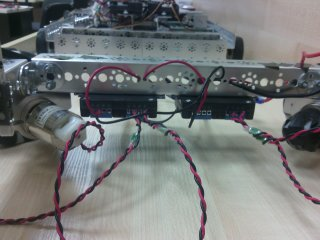
\includegraphics[width=35mm,height=35mm]{Days/3.10.14/3_1_robot}\\ Рисунок 3
			\end{minipage}
			\begin{minipage}{0.3\linewidth}
				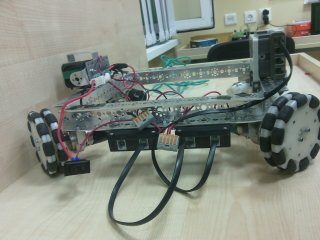
\includegraphics[width=35mm,height=35mm]{Days/3.10.14/3_2_robot}\\ Рисунок 4
			\end{minipage}
			\begin{minipage}{0.3\linewidth}
				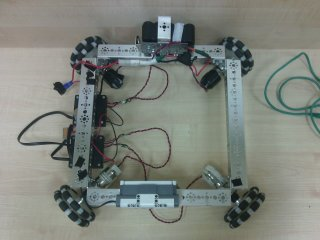
\includegraphics[width=35mm,height=35mm]{Days/3.10.14/3_3_robot}\\ Рисунок 5
			\end{minipage}
		\end{figure}
		\item Идеи и планы для следующего занятия:
		\begin{itemize}
			\item Начать строить механизм захвата и подъема шариков. В качестве механизма подъема можно использовать ножничный подъемник, так как он лёгок в сборке, для поднятий такой конструкции не требуется прикладывать через чур много силы и необходимо небольшое количество материала, чтобы сделать такой ножничный механизм. который будет раздвигаться на большую высоту. Таким образом основными плюсами ножничного подъёника являются простота сборки, быстрота раздвигания механизма(поднятие его над землёй) и высота, на которую он раздвигается. Так же он очень компактен в собранном состоянии. Механизм захвата еще обдумывается. Вероятнее всего это будет резервуар(например корзина), в которую мы сможем помещать шарики с поля и поднимать её на определённую высоту
		\end{itemize}
	\end{enumerate}
	\fillpage
\newpage